%% ----------------------------------------------------------------
%% exam.tex
%% ----------------------------------------------------------------
\documentclass{uosexam2021}    % use option [answers] to include them
%% ----------------------------------------------------------------
\usepackage{graphicx}
%\usepackage{pstricks}
\usepackage{alltt}
\usepackage{amssymb}
\usepackage{amsmath}
\usepackage{amsfonts}
\usepackage{bm}
\usepackage{framed}
\renewcommand{\ttdefault}{pcr}
\newcommand{\tr}{\textsf{T}}
\newcommand{\e}[1]{{\rm e}^{#1}}
\newcommand{\E}[1]{{\rm e}^{{\displaystyle #1}}}
\newcommand{\logg}[1]{\log\left(#1\right)}
\newcommand{\Prob}[1]{\mathbb{P}\left(#1\right)}
\newcommand{\Step}{\mathop{\mathrm{O}\hspace{-15pt}\rule[8.5pt]{11pt}{1.2pt}\hspace{2pt}}}
\newcommand\diag{\mathop{\mathrm{diag}}}
\newcommand{\grad}{\bm{\nabla}}
\newcommand{\dd}{\mathrm{d}}
\newcommand{\class}{\mathcal{C}}
\newcommand{\data}{\mathcal{D}}
\DeclareMathAlphabet{\mat}{OT1}{cmss}{bx}{n}
\newcommand{\pd}[2]{\ensuremath{\frac{\partial #1}{\partial #2}}\xspace}
\newcommand{\M}[1]{\ensuremath{\boldsymbol{#1}}\xspace}
\newcommand{\bst}{\rule{0mm}{5mm}}
\newcommand{\av}[1]{\mathbb{E}\!\left[ #1 \right]}
\newcommand{\seqSeq}[2]{#1{1},\,#1{2},\,\ldots,\,#1{#2}}
\newcommand{\identitySeq}[1]{#1}
\newcommand{\numericalSeq}[1]{\seqSeq{\identitySeq}{#1}}
\newcommand{\subscriptSeq}[2]{{#1}_{#2}}
\newcommand{\sequence}[2]{\seqSeq{\subscriptSeq{#1}}{#2}}
\newcommand{\mpos}[1]{}
\newcommand{\lines}[1]{}
\newcommand{\emptyBox}[1]{}
\newcommand{\inumberedlines}[2]{}
\newcommand{\addspc}{}


\graphicspath{{figures/}}

% \usepackage{picture}
\begin{document}
\unitTitle{Computational Biology}
\authors{Adam Pr\"ugel-Bennett}
\unitcode{COMP3212}
\semester{2}
\year{2020}
\durationhours{2}
\duration{120}

\QtoBeAnswered{Answer all questions. Section~A (worth 40 marks) is a
  series of questions with short answers.  Section~B (worth 60 marks)
  involves longer questions}
\specialInstructions{This examination is worth 70\%. The tutorials was worth 30\%.}

\specialInstructionsBox{}

\addition{0}

\calculator{University approved calculators MAY be used.}


\maketitle

\setlength{\extrarowheight}{3pt}


%\blankpage

%% ----------------------------------------------------------------
\section % A


% ***************************** question 1 **************************
% Compulsory

\begin{question}{40}
  \begin{parts}\mpos{3cm}
    % ******************************
    \part[5]{For Hidden Markov Models (HMMs) describe why
      pseudo-counts are commonly used in training the parameters.}{\lines{6}}
    \begin{answer}
      The emission and transition probabilities are computed from the
      training data, but the training data might be incomplete.  This
      could lead to zero probabilities where in fact there is a small
      probability of an event happening.  Adding pseudo-counts
      prevents any probabilities being zero compensating for using a
      finite training set.
    \end{answer}\mpos{3cm}
    % ******************************
    \part[5]{Describe a good way of encoding different amino acids in
      an artificial neural network.}{\lines{6}}
    \begin{answer}
      Using a one-hot encoding prevents any biases in encoding amino
      acids.  This can be combined with an embedding that may be
      learnt from a different data set.
    \end{answer}\mpos{3cm}
    % ******************************
    \part[5]{Describe what is meant by coalescence in population
      genetics.}{\lines{6}}
    \begin{answer}
      Coalescence occurs when we trace the evolutionary history
      backwards through the generations.  After a certain time
      different genes across the current population have a common
      ancestor.  In asexual reproduction (e.g. in mitrochondrial DNA)
      coalescence will happen relatively rapidly.
    \end{answer}
    \addspc
    \mpos{3cm}
    % ******************************
    \part[5]{What do we mean by conditional independence and why is
      it important in inferring interactions in a gene regulation
      network from correlation data?}{\lines{6}}
    \begin{answer}
      Conditional independence implies that for two random variables
      $X$ and $Y$ when conditioned on a third random variable $Z$ then
      \begin{align*}
        \Prob{X,Y|Z} = \Prob{X|Z}\,\Prob{Y|Z},
      \end{align*}
      this doesn't mean we have full independence $\Prob{X,Y} =
      \Prob{X}\,\Prob{Y}$.  Conditional independence suggests a lack
      of a direct causal link between $X$ and $Y$ despite the fact
      that they be correlated (if they are not fully independent).
    \end{answer}\mpos{3cm}
    % ******************************
    \part[5]{Describe how microarrays are used to measure the
      concentration of RNA.\\}{\lines{6}}
    \begin{answer}
      Microarrays usually consist of a large number of micro-wells
      each containing multiple stands of complementary DNA or RNA.
      Each well would be designed to detect a different RNA.  The
      cells under investigation would have their RNA tagged with a
      fluorescent dye while control cells would have their RNA tagged
      with a different coloured fluorescent dye.  By measuring the
      relative activation of the two sets of cells we can determine the
      relative abundance of RNA strands.
    \end{answer}\mpos{3cm}
    % ******************************
    \part[5]{Explain why we model the time between reaction by an
      exponential distribution.}{\lines{6}}
    \begin{answer}
      The exponential distribution arises from the assumption that in
      any infinitesimal time period the probability of an event is
      independent of any other event and therefore Poisson
      distributed.  The probability of having no events in a
      succession of periods leads to an exponential distribution.
    \end{answer}\mpos{3cm}
    % ******************************
    \clearpage
     \addspc
    \mpos{8cm}
    \part[10]{Below is the finite state automaton modelling affine
      gaps.  Label the transition costs and explain what the three
      states represent.
      \begin{center}
        \includegraphics[width=0.4\linewidth]{fsa_gap-0}
      \end{center}
    }{}
    \begin{answer}
      \begin{center}
        \includegraphics[width=0.4\linewidth]{fsa_gap-1}
      \end{center}
      \begin{description}
      \item[$M$] represents the case where there is no gap and the
        amino acids are being substituted
      \item[$I_a$] corresponds to a gap where we insert into
        string $\bm{a}$
      \item[$I_b$] corresponds to a gap where we insert into
        string $\bm{b}$
      \end{description}
    \end{answer}
  \end{parts}
\end{question}
\addspc
%\clearpage

%% ----------------------------------------------------------------


\section % B
\newcommand\mycom[2]{\genfrac{}{}{0pt}{}{#1}{#2}}


% ***************************** question 2 **************************
% Suffic Tree

\begin{question}{20}
  \begin{parts}\mpos{2cm}
    \part[5]{Write down all the suffixes of the string
      ``\textbf{GTAACGT\$}''.}{\lines{2}}
    \begin{answer}
      \{\$, T\$, GT\$, CGT\$, ACGT\$, AACGT\$, TAACGT\$, GTAACGT\$\}
    \end{answer}
    \mpos{6cm}
    \part[10]{Sketch the suffix tree (trie of all suffixes) for
      ``\textbf{GTAACGT\$}''.}{\emptyBox{10}}
    \begin{answer}
      \includegraphics[angle=270,width=0.9\linewidth]{Suffixes.png}
    \end{answer}\mpos{2cm}
    \part[5]{How many comparisons are necessary to find a match to
      the string ``\textbf{ACG}'' in ``\textbf{GTAACGT\$}'' using the
      suffix tree.}{\lines{2}}
    \begin{answer}
      Two comparisons are necessary to reach a leaf.
    \end{answer}
  \end{parts}
\end{question}

\addspc
%\clearpage


% ***************************** question 3 **************************
% Needleman-Wunsch

\begin{question}{20}
  Using the Blosum50 substitution matrix
  \begin{center}
    \includegraphics[width=0.55\linewidth]{blosum50}
  \end{center}
  \begin{parts}\mpos{4cm}
    \part[10]{Complete the following table for Needleman-Wunsch
      algorithm using a cost of $d=8$ for gaps.
      \begin{center}
        \includegraphics[width=0.6\linewidth]{nW-0}
      \end{center}
    }{}
    \begin{answer}
      \begin{center}
        \includegraphics[width=0.6\linewidth]{nW-1}
      \end{center}
    \end{answer}
    \part[10]{Show the path followed by the backward algorithm for
      Needleman-Wunsch and show the corresponding match for the two
      sequences shown below.
      \begin{center}
        \includegraphics[width=0.75\linewidth]{needlemanWunschA-0}
      \end{center}
    }{}
    \begin{answer}
      \begin{center}
        \includegraphics[width=0.75\linewidth]{needlemanWunschA-1}
      \end{center}
    \end{answer}
  \end{parts}
\end{question}


\addspc
%\clearpage


% ***************************** question 4 **************************
% Dynamical Systems
\newcommand{\goesto}[1]{\stackrel{#1}{\longrightarrow}}

\begin{question}{20}
  \begin{parts}\mpos{4cm}
    \part[5]{Write down the ordinary differential equations (ODEs)
      describing the set of chemical equations
      \begin{align*}
        Y &\goesto{k_1=1} X + Y  & 2\,X &\goesto{k_2=1} 2\,X + Y\\
        X &\goesto{k_3=1} \varnothing & Y &\goesto{k_4=1} \varnothing.
      \end{align*}
      }{\lines{5}}
    \begin{center}
    \end{center}
    \begin{answer}
      ODEs
      \begin{align*}
        \frac{\dd [X]}{\dd t} &= [Y] - [X]\\
        \frac{\dd [Y]}{\dd t} &= [X]^2 - [Y]
      \end{align*}
      Nullclines are given by $[Y]=[X]$ and $[Y] = [X]^2$ with a fixed
      point at $[X]=[Y]=1$
    \end{answer}
    \part[5]{Sketch the nullclines on the axis shown and mark the
      position of the second fixed point other than $[X]=[Y]=0$.
      \begin{center}
        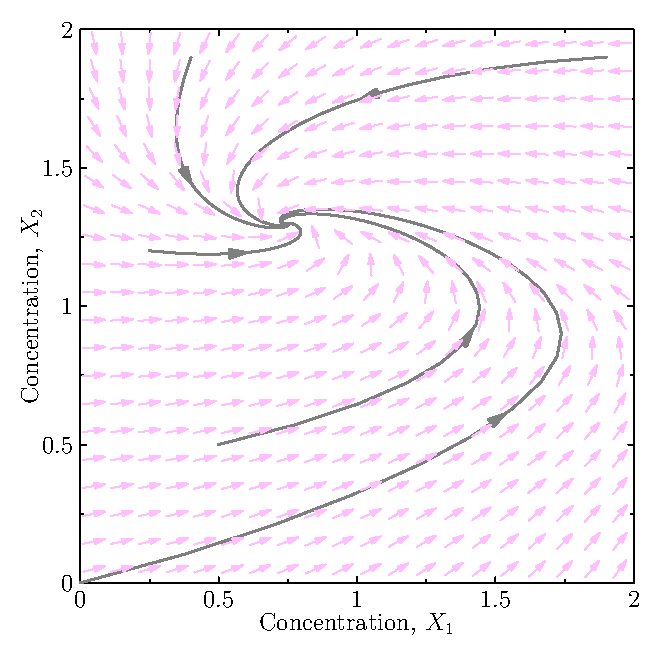
\includegraphics[width=0.39\linewidth]{nullclines-0}
      \end{center}
    }{}
    \begin{answer}
      \begin{center}
        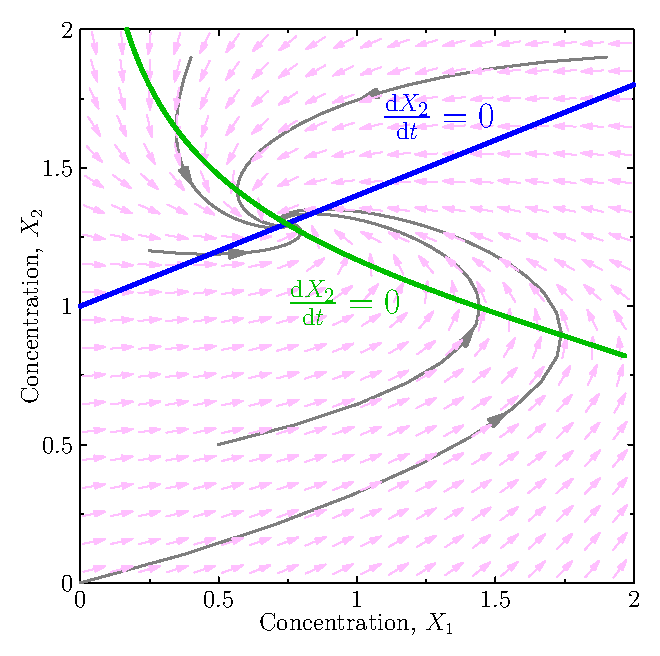
\includegraphics[width=0.39\linewidth]{nullclines-1}
      \end{center}
    \end{answer}
%    \clearpage\mpos{6cm}
    \part[10]{Compute the Jacobian at the fixed point.Using the fact that the eigenvalues of a
      $2\times2$ matrix,
      \begin{align*}
        \mat{J} =
        \begin{pmatrix}
          J_{11} & J_{12} \\
          J_{21} & J_{22}
        \end{pmatrix}
      \end{align*}
      are equal to
      $\lambda_{1,2} = T/2 \pm \sqrt{T^{2}/4-D}$ where
      $T = \mathop{\mathrm{tr}} \mat{J} = J_{11} + J_{22}$ and
      $D= \det(\mat{J})=J_{11}\,J_{22}-J_{12}\,J_{21}$ compute the
      eigenvalues of $\mat{J}$ and comment on the stability of the fixed
      point.}{\lines{10}}
    \begin{answer}
      \begin{align*}
        \mat{J} =\left.
        \begin{pmatrix}
          -1 & 1\\
          2\,X & -1
        \end{pmatrix}\right|_{([X],[Y])=(1,1)}
                 =
                 \begin{pmatrix}
                   -1 & 1\\
                   2  & -1
                 \end{pmatrix}
      \end{align*}
      So that $D=\det(\mat{J}) = -1$ and $T = \mathop{\mathrm{tr}}
    \mat{J} = -2$. Thus $\lambda = -1 \pm \sqrt{2}$ and the fixed
    point is unstable as one of the eigenvalues is greater than 0.
    \end{answer}
  \end{parts}
\end{question}

\addspc
\clearpage




% ***************************** End of exam *****************************
\end{document}



%%% Local Variables:
%%% End:
